\section{\texttt{Current work}}
\begin{frame}{\textbf{Saliency Estimation}}
\begin{columns}
	\begin{column}{0.48\textwidth}
		\begin{varblock}[\textwidth]{Objective}
			To identify pixels that are quite distinct and grabs attention.
		\end{varblock}
	\end{column}
	\begin{column}{0.48\textwidth}
	\begin{varblock}[\textwidth]{Techniques}
		\footnotesize
		\begin{multicols}{2}
		\begin{itemize}
    			\item Hierarchical Color Based
		    \item Context Aware Based
    			\item Spectral Distribution Based
    			\item Regional Contrast
		\end{itemize}
		\end{multicols}			
	\end{varblock}
	\end{column}
\end{columns}
	\begin{figure}
		\centering
		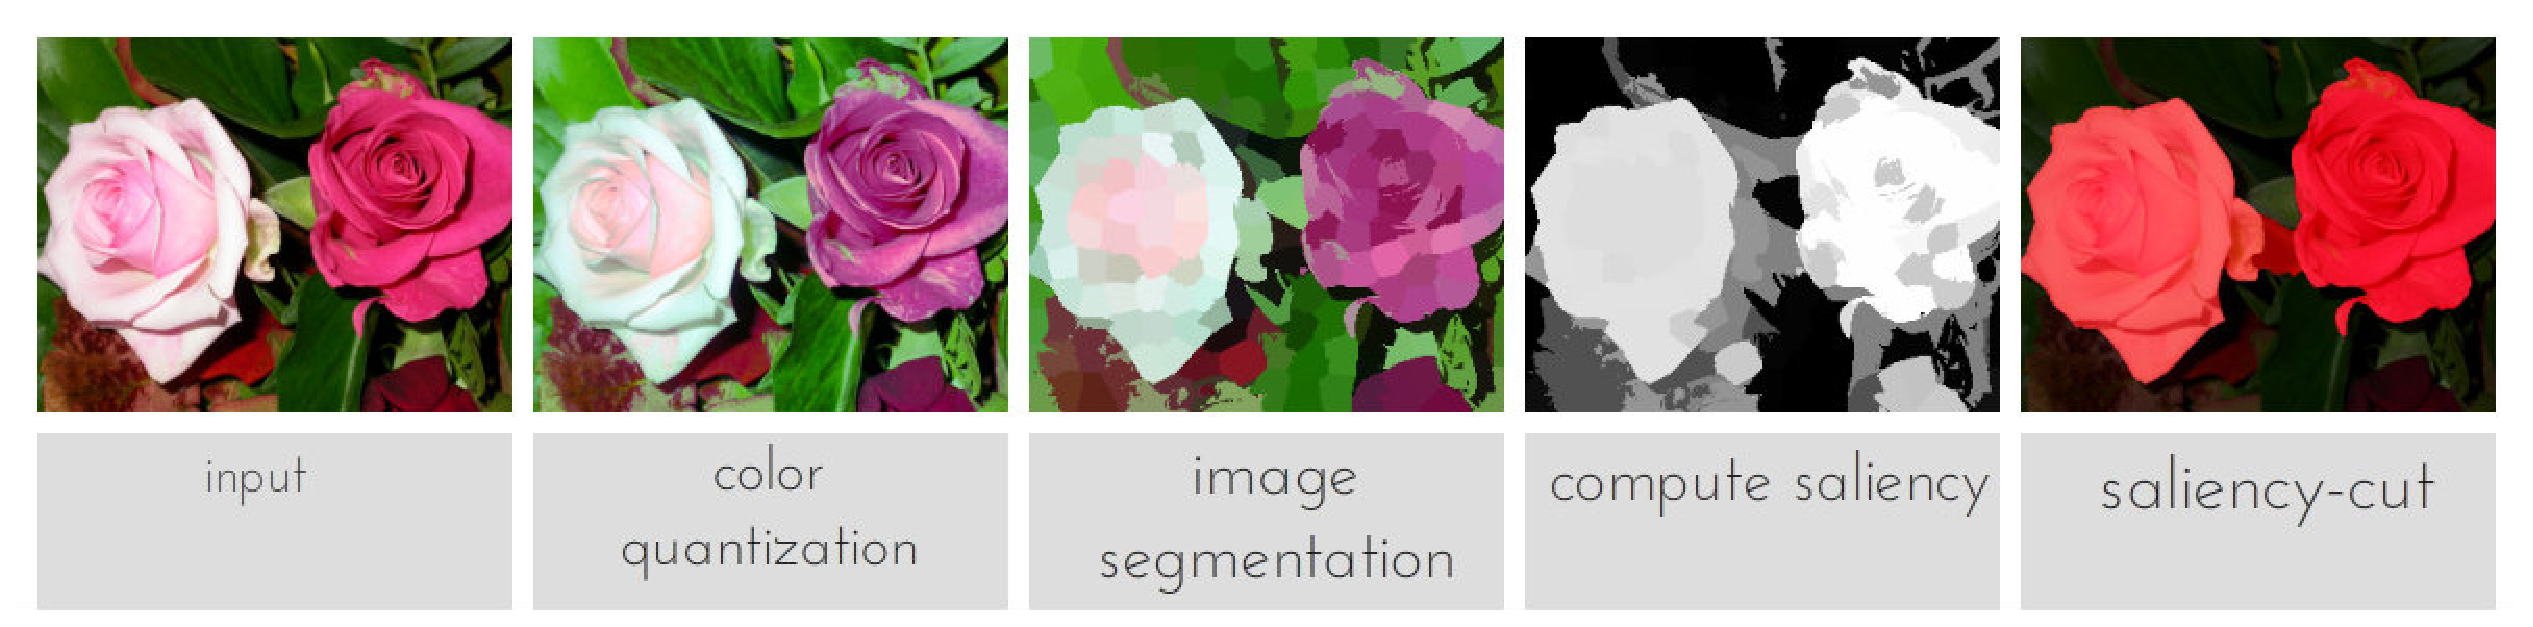
\includegraphics[width=0.7\textwidth]{./img/saliency.eps}
		\caption{A general approach for saliency estimation.}
	\end{figure}
\end{frame}